\documentclass[10pt,a4paper]{report}

\usepackage{multirow}
\usepackage{graphicx}
\usepackage{fancyhdr}
\usepackage{listings}
\usepackage{xcolor}
\usepackage[Glenn]{fncychap}
\usepackage[hang,small,bf]{caption}

% -- Hyperlinks settings -------------------------------------------------------
\usepackage{hyperref}
\hypersetup{
    colorlinks,
    citecolor=black,
    filecolor=black,
    linkcolor=black,
    urlcolor=black
}

\pagestyle{fancy}
\fancyhf{}
\fancyhead[RO]{\small \thepage}
\fancyhead[LO]{\textit{\small \nouppercase{\leftmark}}}

% -- Document begin ------------------------------------------------------------
\begin{document}

\title {
    \scshape
    \huge 
        Real-Time Systems project v1.0\\[5mm]
        \hrule
}
\author {
    \textsf{Alberto Franco} \\
    \textsf{afranco87@gmail.com}
}
\date {
    \sffamily
    \small
    PDF generated on \today
}
\maketitle % -- end Title ------------------------------------------------------

%--- LISTING SETTINGS ---------------------------------------------------------%
\definecolor{darkgray}{rgb}{0.97,0.97,0.95}
\definecolor{darkgreen}{rgb}{0.0, 0.6, 0.0}
\definecolor{gray}{rgb}{0.2,0.2,0.3}
\definecolor{fuchsia}{rgb}{0.6, 0.0, 0.95}
\definecolor{darkred}{rgb}{0.6, 0.0, 0.0}

\lstset{language=Ada}
\lstset{backgroundcolor=\color{darkgray}}
\lstset{keywordstyle=\color{blue}\ttfamily}
\lstset{basicstyle=\color{gray}\ttfamily\footnotesize}
\lstset{commentstyle=\color{darkgreen}\ttfamily}
\lstset{stringstyle=\color{darkred}}
\lstset{showstringspaces=false}

% \lstset{numbers=left}
\lstset{numberstyle={\ttfamily\footnotesize}}
\lstset{firstnumber=last}

\lstdefinelanguage{mast}
  {morecomment=[l]{--},
   morestring=[b]",
   morestring=[d]'
  }
%------------------------------------------------------------------------------%

\setcounter{page}{1}
\pagenumbering{roman}

\tableofcontents
\newpage

\chapter*{Change Record}

\paragraph{Version 1.0:}
Added \emph{Task description} section. Revision of chapters 1 to 4. 

\paragraph{Version 0.6:}
Revision of chapter 4. Changed sustainability plots and update of sensitivity 
analysis. 

\paragraph{Version 0.5:}
Partial rewrite of chapter 4. Changed analysis procedure, updated data to be 
consistent with the new analysis done. 

\paragraph{Version 0.4:}
Added chapter 4 about system analysis. It describe system analysis. 
Corrections in chapter 2 and 3.

\paragraph{Version 0.3:}
Added chapter 3 about mode change. It describe mode-change protocol. 
Corrections in chapter 2.

\paragraph{Version 0.2:}
Added chapter 2 about software architecture. It describe which type of tasks we
have in the software system and how they interact and collaborate with each 
others and with the user. 

\paragraph{Version 0.1:} 
Document creation, added preliminary analysis chapter describing what type of 
system we want to create and a brief introduction on the topic. 

\newpage
\setcounter{page}{1}
\pagenumbering{arabic}

% -- end Bureaucracy section -----------------------------------------------------

\chapter{Preliminary analysis}
This initial chapter introduces the topic and provide an outline of the system 
under analysis. We want to design a simple simulator of a control software of a 
nuclear plant. The focus will be on second-generation plants (Pressurized water 
reactors) since they are simpler to understand but still present some 
non-trivial behavior and they are interesting to deal with. The rest of this 
chapter is organized as follows: first we  introduce the operations of a plant 
and its critical issues and problems; second, we draw some system requirements 
and finally we give a high level ideas on how the software should behave 
in operation.

% ------------------------------------------------------------------------------
% -- Plant description section
% -- 
\section{Description of a $2^{nd}$ generation nuclear plant}
A nuclear plant transforms energy produced from nuclear fission into heat and 
then, through an alternator, into electrical energy. This is done via heat 
exchange and steam-powered turbines. Figure \ref{nuclearimg} depicts
the plant. \emph{Reactor vessel} contains nuclear fuel (Uranium-235 for this 
type of reactors) that produces energy through nuclear fission. This energy is 
convolved through water in \emph{reactor circuit} as heat that is exchanged to 
\emph{turbine circuit}. In the turbine circuit water is converted into steam 
that makes the turbine operational. Turbines are connected to alternators that 
produce alternate current. After steam has passed through turbines it is cooled 
to be re-pumped into the circuit. Cooling is done by exchanging heat with 
\emph{cooling circuit} that keeps water temperature low using cooling tower that 
are the popular image associated with nuclear plants.
\begin{figure}[htb]
\centering
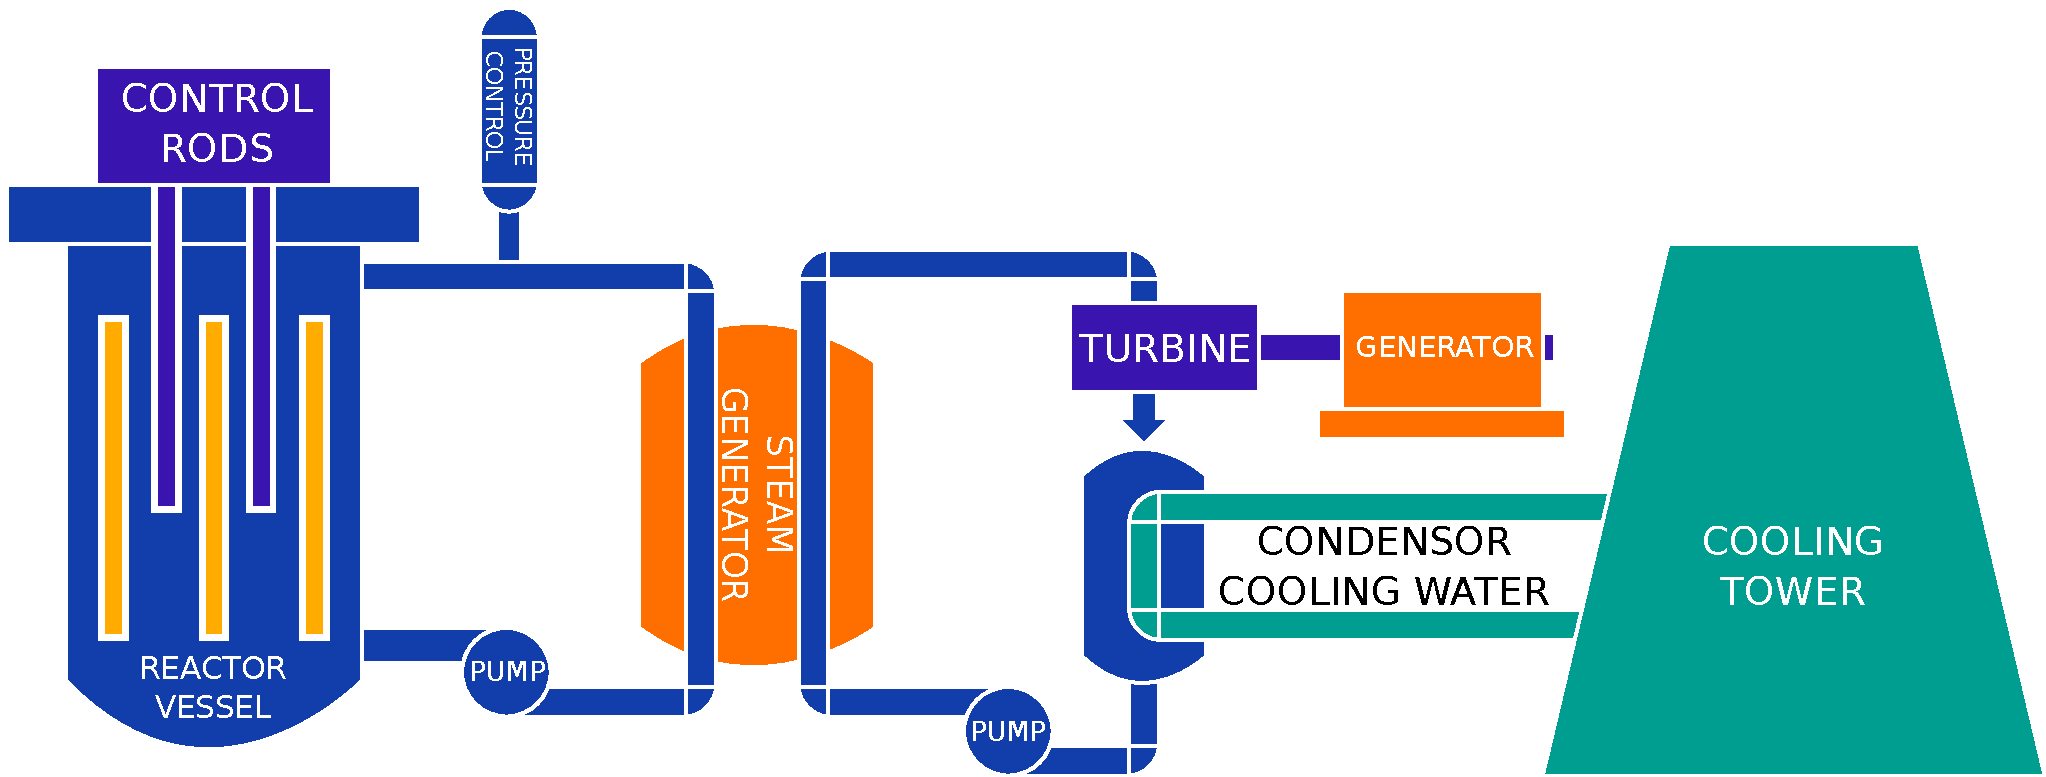
\includegraphics[width=\textwidth]{images/Nuclear_Plant}
\caption{Plant simplified depiction}
\label{nuclearimg}
\end{figure}

\emph{Control rods} are used for preventing the reaction from being devastating. 
Without those rods the reactor would be an atomic bomb. The more control 
rods are inserted into the core the less the reaction produce energy. Rods are 
composed of materials capable of absorbing many neutrons, the particles 
that trigger nuclear fission. Reaction is controlled via progressive insertion 
of control rods into the core, up to a complete shutdown of the core through 
total insertion of the rods into the core. 

We have to keep in mind a few critical issues with the system. In this 
kind of plant once operation has started it is nearly impossible to stop. 
Whereas control rods are used to reduce reaction speed also with complete 
immersion reaction continues for one to three years. In essence, cooling water
must be pumped up to shutdown completion. 

\subsection{Critical issues}
All safety-critical issues are related to reactor circuit. Water must be 
pressurized and pumped at all time, even when the reactor has been shutdown.
This will heavily impact software design. There must be no water leakage from the
reactor circuit since water is used as moderator of fission reaction and it 
is in direct contact with uranium pellets, which makes it radioactive. Control 
rods must be under safety limits at all the time, excessive extraction of rods 
from the core lead to meltdown\footnote{
    As an example, Chernobyl disaster happened due to
    an human error. In that plant, control rods were not enough immersed into the
    core in order to raise efficiency.
}. Water inside the circuit must not boil, it is kept so using pressure control
devices. Since we know the properties of the water, we can calculate the exact 
boiling point of water at a given pressure. These are requirements that must be 
satisfied also after plant shutdown. 

Other issues are related with plant efficiency, the main difference with previous
issues is that those are not safety-critical so may not lead to a nuclear disaster.
All pumps must be operational in order to ensure plant operations, temperature
into the turbine circuit must be high enough to convert water into steam and
in cooling circuit low enough to do the opposite. Those requirements must be 
fulfilled to keep the plant running efficiently. 

% ------------------------------------------------------------------------------
% -- Software requirements section
% -- 
\section{System requirements}
The software system we want to design must ensure plant operations and safety. 
System activity must be carried out in a real-time fashion since malfunctions 
may lead to irreversible aftermath. In this section we identify the main software 
requirements that determine system design. Each requirement is categorized by 
importance on a critical-based approach. At the end of this document we provide
a taxonomy of tasks that system should carry out, ordered by importance. In 
this preliminary analysis we draw only requirements that are strictly compulsory.

First we introduce the most critical requirements that are safety-related. These
few controls ensures that the system will always operate under safety conditions.
From this table we derive architectural component that accomplish that kind of 
tasks.
\begin{center} 
% ------------------------------------------------------------------------------
% -- SAFETY-CRITICAL REQUIREMENTS
% -- 
\begin{tabular}{| p{10cm} |}
\hline
\textbf{Safety-critical requirements}\\
\hline \hline
Maintain control rods level under safety limits.\\
\hline
Maintain water pressure in reactor circuit at an appropriate level based on 
his actual temperature and under pipe-resistance safety level.\\  
\hline
Shutdown core and signal malfunction if there is water leakage on reactor circuit.\\ 
\hline 
Do not allow meltdown at any time.\\
\hline
\end{tabular}
\end{center}

Next we have operational requirements. These requirements ensure correct plant 
behavior, although they are not as critical as the previous ones. Oscillations of 
the output power are tolerated in some limits. Here we note that the system must
support different operation modes. 
\begin{center}
% ------------------------------------------------------------------------------
% -- OPERATION-CRITICAL REQUIREMENTS
% -- 
\begin{tabular}{| p{10cm} |}
\hline
\textbf{Operation-critical requirements}\\
\hline \hline
Maintain an appropriate temperature of the core in order to ensure that water 
convert into steam and allow turbine operations.\\
\hline
Maintain apparatus functionality at all the time. \\ 
\hline
On plant full operations, maintain output power inside a given range.\\
\hline
Maintain a temperature in cooling circuit as low as it is required to condense 
steam to water. \\
\hline
\end{tabular}
\end{center}

Last we identify some requirements to serve user operation and mode changes. 
We want to build a self-preserving system, this means that we allow user
to ask for some operations to be carried out but we do not ensure that those 
operations will be carried out if they lead to potential problems.
\begin{center}
% ------------------------------------------------------------------------------
% -- USER INTERACTION REQUIREMENTS
% -- 
\begin{tabular}{| p{10cm} |}
\hline
\textbf{User interaction requirements}\\
\hline \hline
User must be able to select and adjust power output.\\
\hline
User must be able to shutdown the plant.\\
\hline
User must be able to receive information about system operations.\\
\hline
System must be able to go in maintenance mode without shutting down to allow 
users to change non-critical parts of the plant.\\
\hline
\end{tabular}
\end{center}

We must ensure that all these requirements are fulfilled by the software 
system that we are going to design. In the next section we go a bit more
into details on which components are needed, on how every part should be tied up 
and its relationship with other components.

% ------------------------------------------------------------------------------
% -- System activities section 
% -- 
\section{System activities}
This section identifies various activities that must be performed in order to 
fulfill the above requirements. We separate those activity in two main 
categories: \emph{time-triggered} and \emph{event-triggered}. This separation is 
reflected in the actual design: time-triggered activities map to periodic 
tasks and event-triggered map to sporadic tasks. We do not allow aperiodic 
tasks to ensure a better schedulability of the system.

\subsection{Operation modes}
We have four different operation modes. Each mode reflect a specific 
phase of plant life cycle. We support through software:
\begin{itemize}
    \item \textbf{Start mode.} When the plant be asked to start, all its 
    processes need a certain amount of time to become fully operational.
    \item \textbf{Operational mode.} This is the normal mode, possibly will
    last for the entire life cycle of the plant. 
    \item \textbf{Maintenance mode.} Tightly similar to start mode keep 
    some basic services alive and allow user to perform maintenance operations.
    \item \textbf{Shutdown mode.} Once the software is booted up is in 
    shutdown mode. Activity in this mode satisfies only safety-critical 
    requirements.
\end{itemize}
We present a simple state diagram that show how modes are interconnected. 
Each transition is related to a specific events that may be automatically
triggered or requested by the user. Obviously the system never shutdown on his
own. Complete software shutdown is not acceptable.
\begin{figure}[htb]
\centering
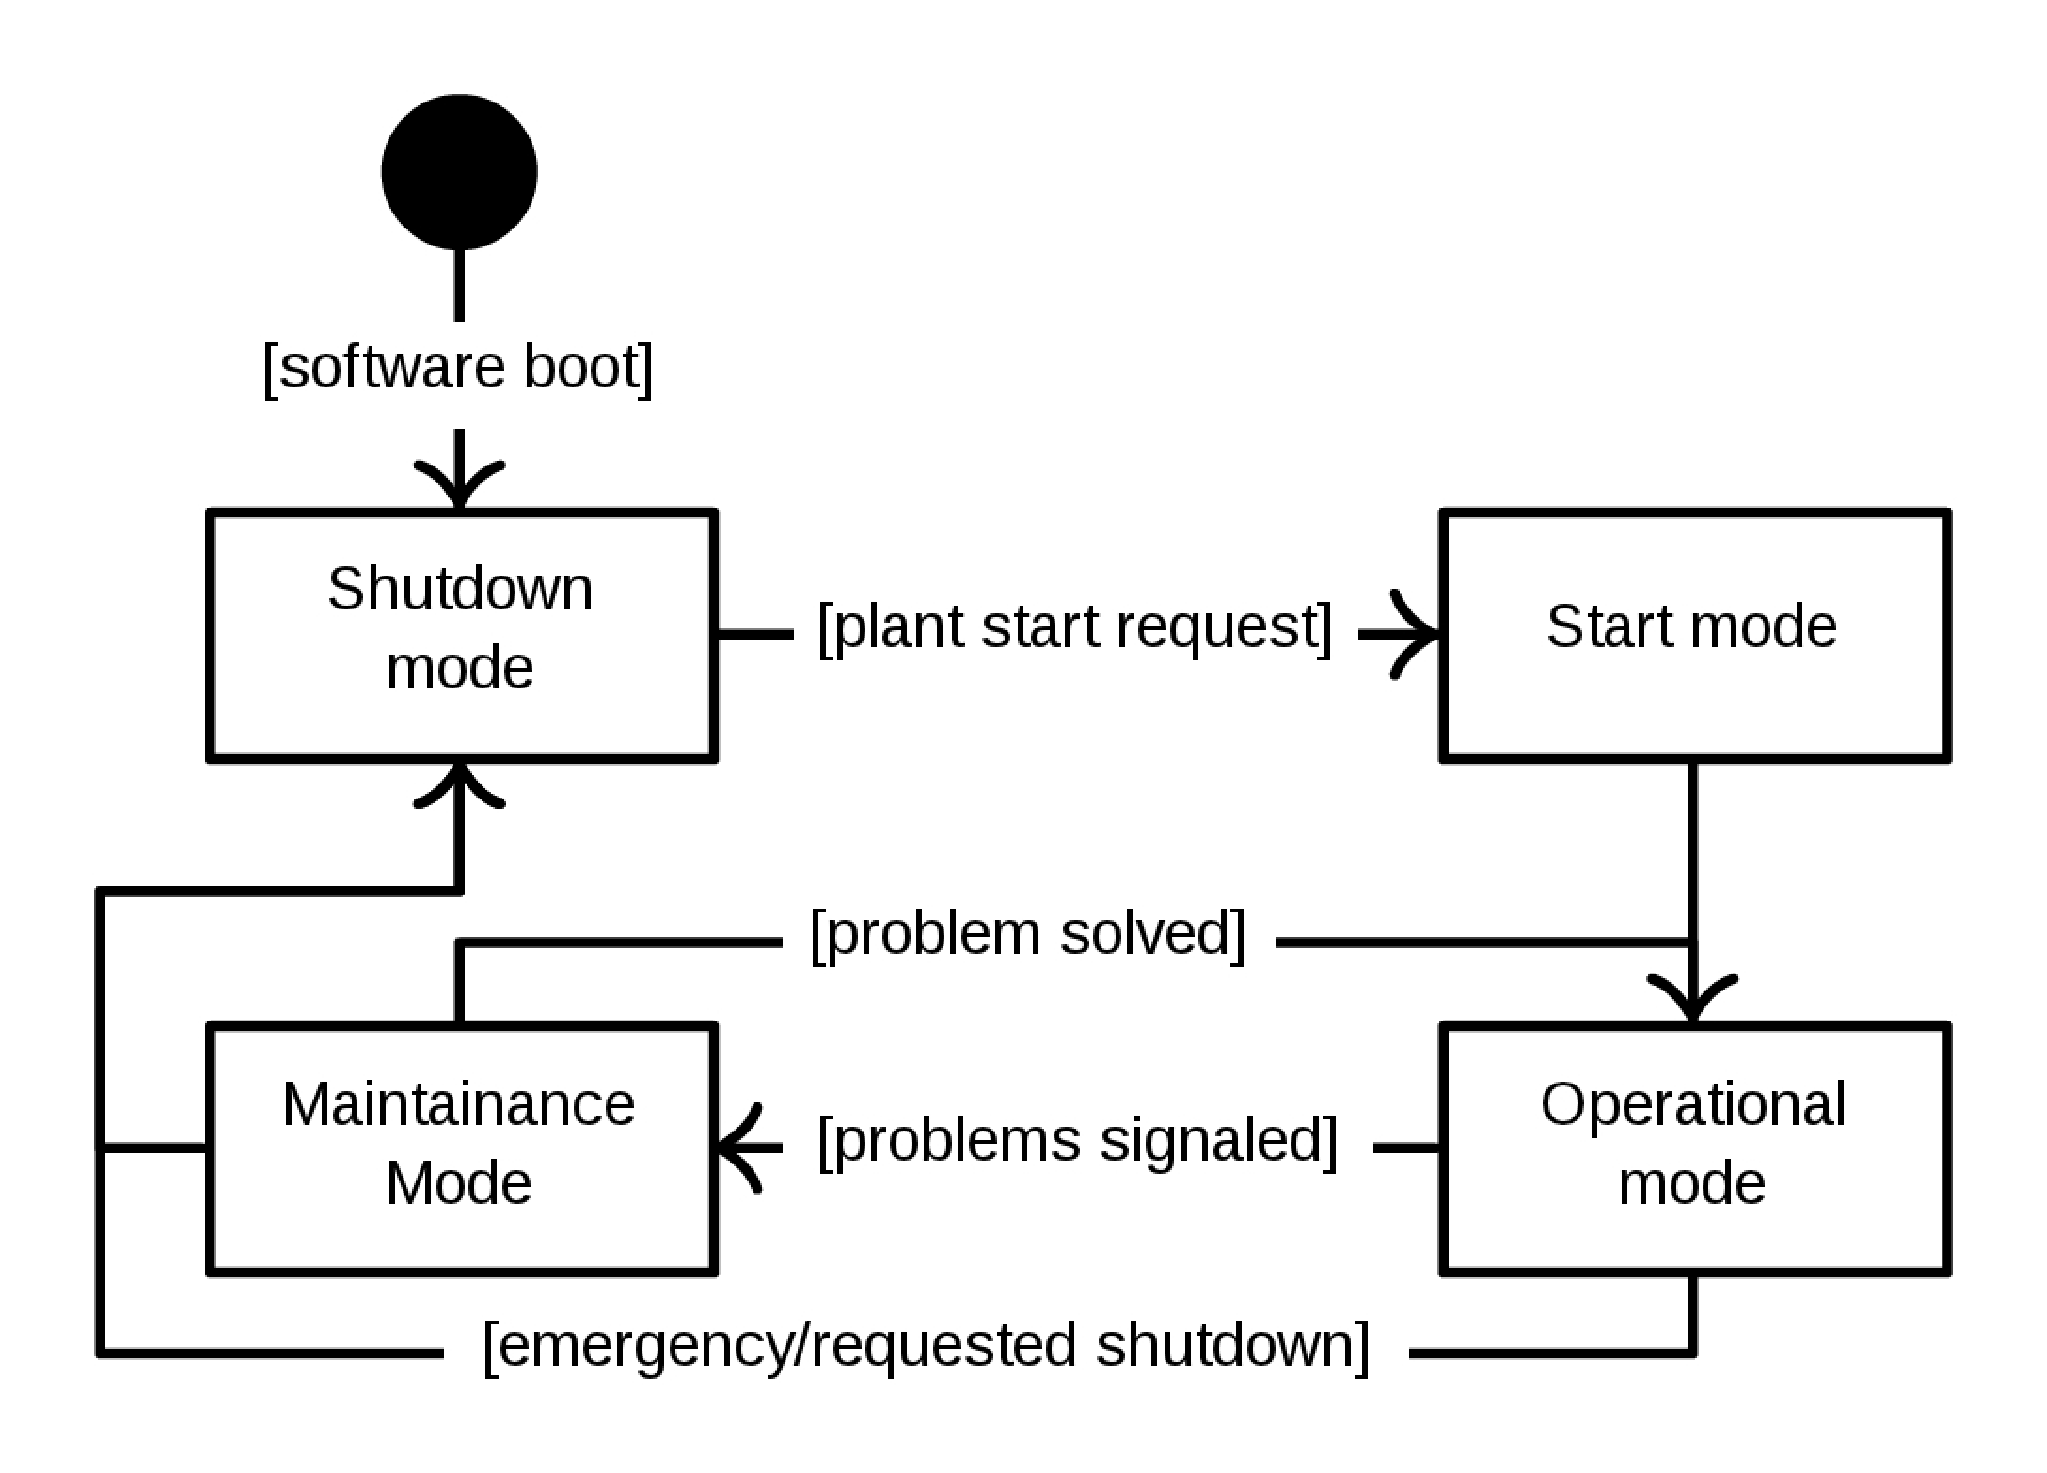
\includegraphics[width=0.6\textwidth]{diagrams/OpModes}
\caption{System Mode Diagram}
\end{figure}

In the fully operational state the system will performs several checks about all
machineries that allow the correct behavior of the plant. All this checking 
operation is to be time-triggered at constant period. If an anomalous situation 
is found it is signaled to an actuator that attempts to repair or signal or 
eventually shuts the plant down. Figure \ref{sysbackactive} shows all background 
checking activity with the signal to actuator relative to that specific issues. 
Those activities have been split into two separate tasks, one for safety-critical 
checks and the other for operational-critical checks.
\begin{figure}[htb]
\centering
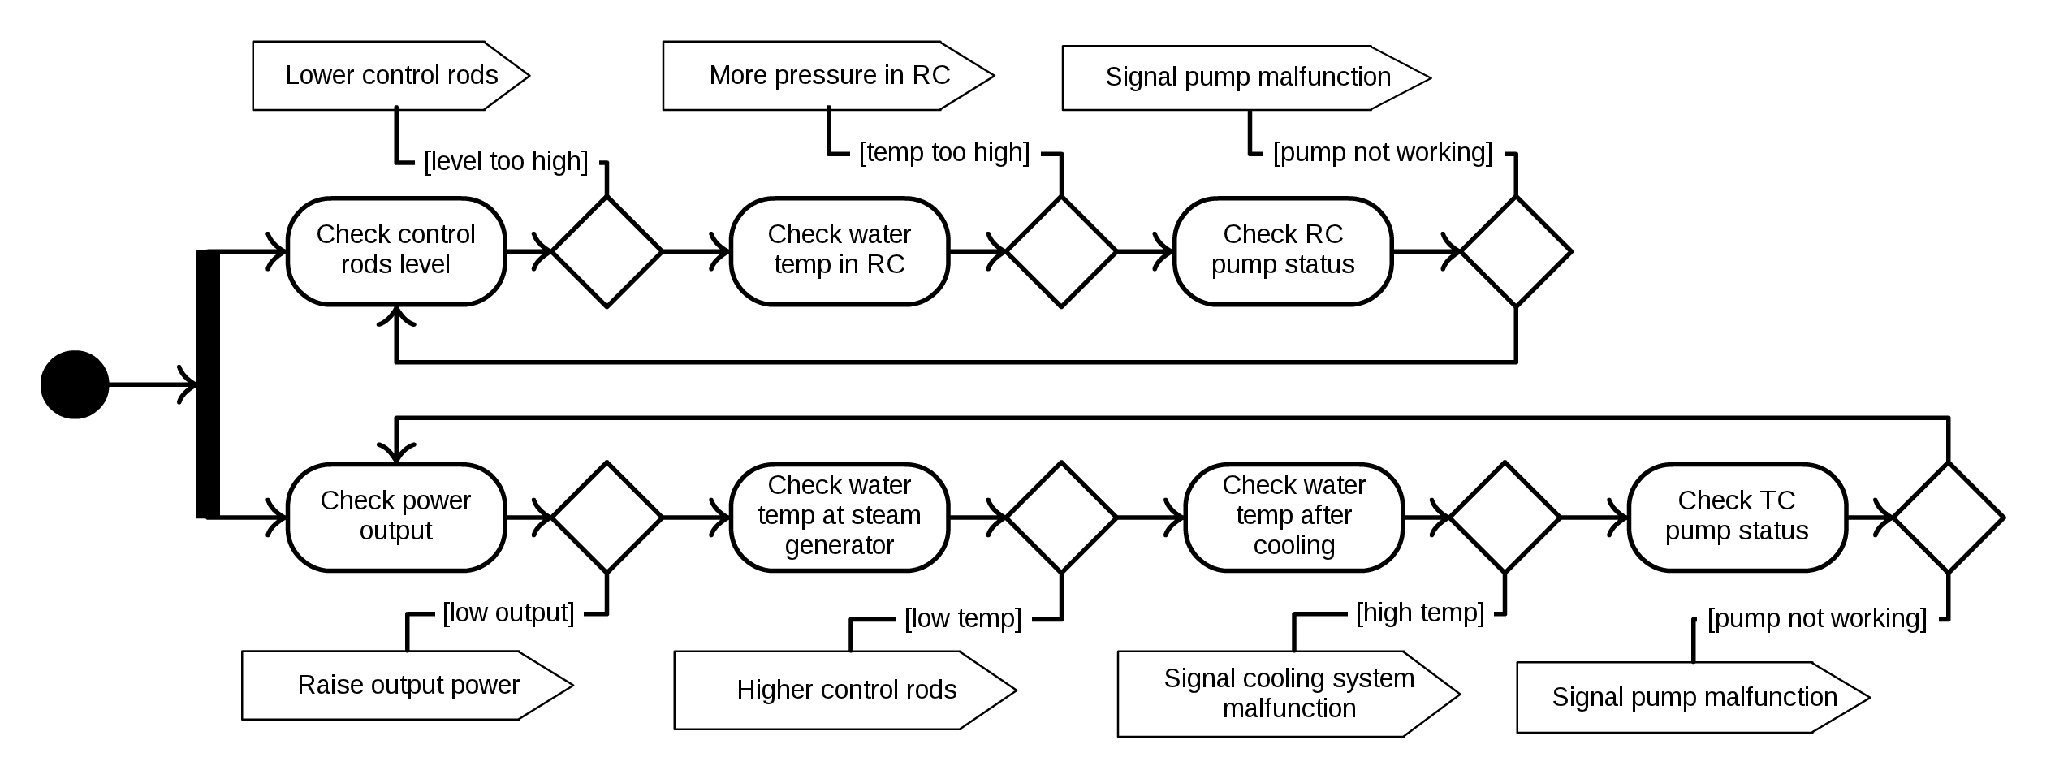
\includegraphics[width=\textwidth]{diagrams/Arch_Activity}
\caption{System background activities}
\label{sysbackactive}
\end{figure}
Other activities are performed on request by the user. This may include
mode change or output power adjustment. Those user operations are performed 
always conservatively. 

Other operation modes are quite similar between them, they all guarantee basic 
functionality of the plant and make it possible to perform some actions. Start 
mode is quite simple, it lets the system start and continue to check for correct 
operation of critical apparatus (as in the shutdown mode). Maintenance mode does 
the same but has a lower restore time since it stops only services that undergo 
maintenance.

\section{Reflections}
Before closing this chapter we want to make some further observations on how 
we want to carry out the task of designing and implementing this system. The 
idea is not to implement a complex simulation that respects tightly the physics
rules that control nuclear reactions, it is just a way to dive into critical 
system design and to get a feel of it. This will not totally discard the 
intrinsic complexity that stands behind this topic. Most of the time we 
will address some topics about which we do not have enough expertise. In 
real-world scenarios the design of such a software system is performed jointly 
by a team of experts. 

% ------------------------------------------------------------------------------
% -- Software architecture chapter
% --
\chapter{Software Architecture}
In this chapter we describe the system architecture through a series of 
specifications and diagrams. We introduce first some formalism that
we use throughout this document. After that we enumerate and describe 
all of the software components designed and we point out the connections 
between components. We describe how resources are accessed and how 
communication with users is carried out. At the end of the chapter we provide a 
brief summary.

\section{Workload model and Task archetypes}
We are going to use sporadic workload model for system design. We have periodic
task and sporadic tasks but no aperiodic task. Periodic tasks are so inside 
operational modes that we discuss later on. Sporadic tasks have a minimum 
interarrival time between activations. Once the task is active it issue a 
\emph{job} that perform the work it has been design to do. 

We define a few archetypes for tasks to use in the design of the software 
system. Periodic tasks are considered so only inside operational mode. It will 
become clear to the reader that due to the use of different operation modes 
those tasks are to be triggered by a coordinator. Figure \ref{periodicarch} 
depicts, with a component diagram, periodic archetypes. 
\begin{figure}[htb]
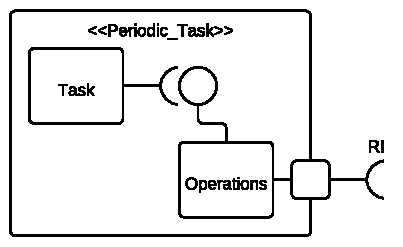
\includegraphics[width=0.5\textwidth]{diagrams/Periodic_Components}
\centering
\caption{Periodic components archetypes}
\label{periodicarch}
\end{figure}    

Then we have sporadic components that behaves as expected. Sporadic jobs are 
triggered by events generated by external sources or other jobs. They have a 
minimum inter-arrival time and never arrive sooner than that time. We do not
allow aperiodic jobs in the design of this software system.
\begin{figure}[htb]
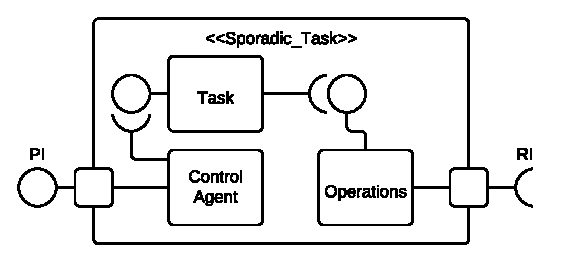
\includegraphics[width=0.6\textwidth]{diagrams/Sporadic_Components}
\centering
\caption{Sporadic components archetype}
\end{figure}
The reader may notice that we have marked each diagram that represent a task 
archetype with a UML stereotype. Hereafter we use those stereotypes to denote 
that we are referring to that type of tasks, not to burden too much diagrams 
with overwhelming notation. 


% ------------------------------------------------------------------------------
% -- Architecture definition section
% --
\section{Task definition}
In this section we describe each task and its interaction with other 
components of the system. We use UML sequence diagrams to describe 
interactions between components. All of the sequence diagrams presented here are 
worst-case execution scenarios, most of the times the messages that we depict in
sequences will not be sent. 

\paragraph{On operational modes. }
While reading the next sections one should notice that there are no sharp 
differences between operational modes. \texttt{Start\_Mode} and 
\texttt{Operational\_Mode} are merged in the software by design. This is done 
because there is logical distinctions but it is senseless to introduce an 
operational mode that does nothing and a start mode that fine tunes components of 
the plant and switch constantly between the two.

\texttt{Maintenance\_Mode} and \texttt{Shutdown\_Mode} have just few differences
in control rods status. Here also there are very few differences between the two
modes but they are not just logically separated but designed as two different 
modes. During this chapter we do not focus on the protocol that manage mode 
change. We go into more details about mode change in the next chapter.

\subsection{Periodic tasks}
The system must take care of few critical components, whose status must be checked
throughout the plant life cycle. Those are related to reactor circuit (RC from now 
on, for sake of brevity) and perform status checking of core apparatus. Figure
\ref{coretask} depicts how periodic tasks collaborate with relevant actuator tasks.
We denote with the term \emph{actuator tasks} some kind of sporadic tasks 
that communicate with the physical actuators. 
As stated in previous chapter we have to perform three core checks for RC. First
we need to check control rods immersion level, second we need to check the water 
temperature, if it is too high we need to higher pressure or lower control rods 
to prevent water from boiling. Last we need to check pump functionality and 
report to users in case of problems. Here we identify also some sporadic 
tasks, mostly actuators tasks. The system must provide actuators for both, 
control rods and water pressure in RC, that respond to status-checking-tasks 
stimuli. Another sporadic task that we identify here is system notification pipe 
that inform users of errors that require human intervention and properly change 
operational mode. These tasks are strictly periodic, in the sense that they 
are active in all operational modes of the plant to ensure safety at all the time. 
\begin{figure}[htb]
\centering
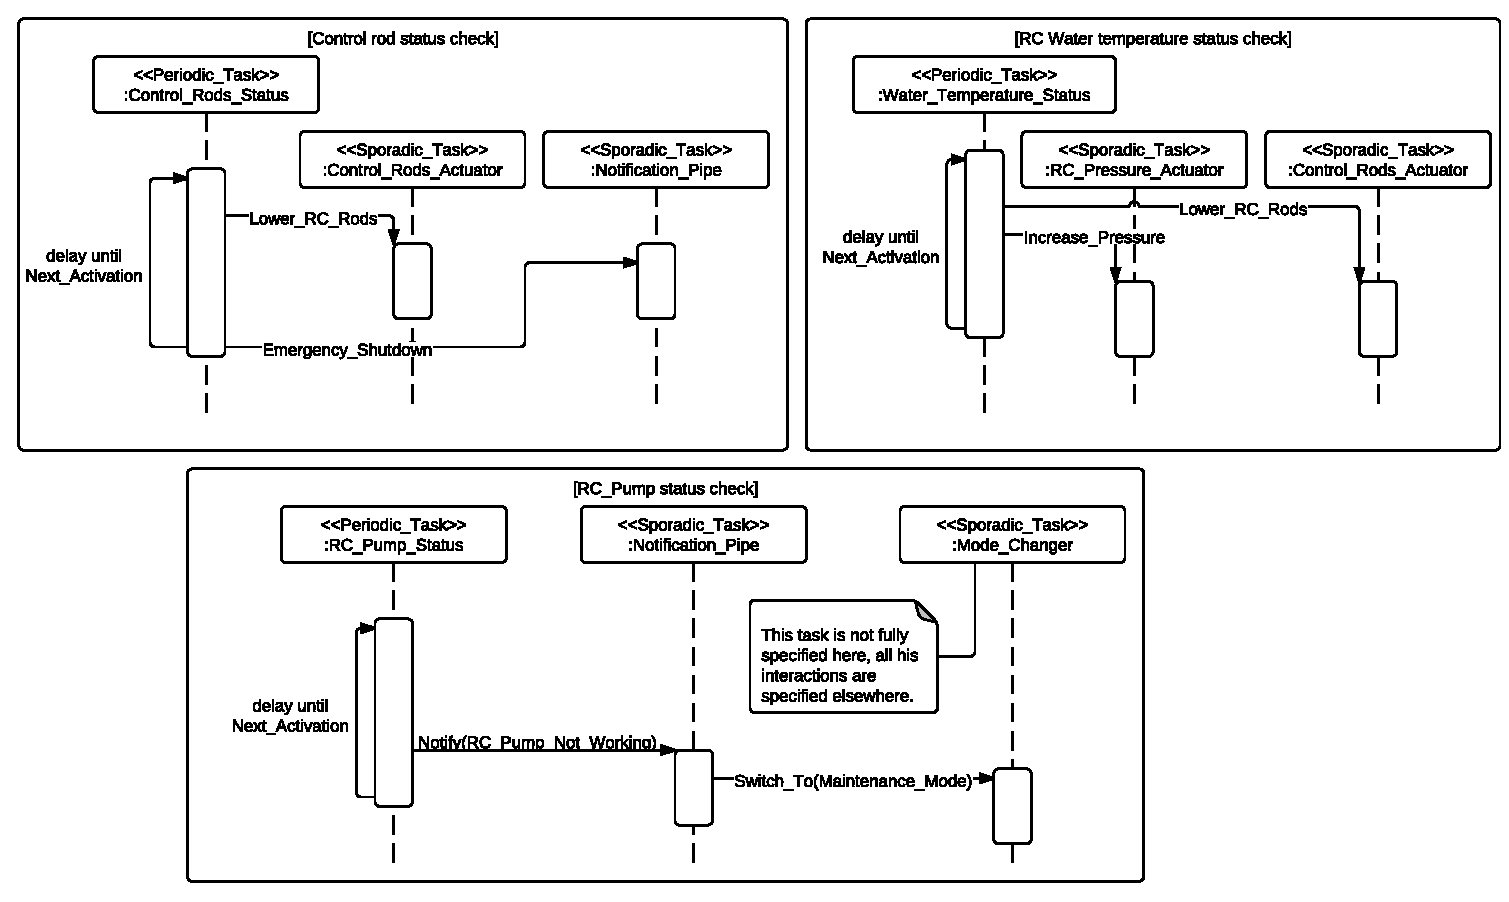
\includegraphics[width=\textwidth]{diagrams/RC_Status_Diagram}
\caption{Task for core apparatus checking}
\label{coretask}
\end{figure}

Checking tasks in RC performs operation always conservatively, i.e. they never 
move the plant to a potentially dangerous status. Last thing to notice is that 
the \texttt{Mode\_Changer} task is not fully specified in this diagram. Exploiting 
its behavior would require a complex and barely-readable diagram that we do not 
present. Away from what its depicted once \texttt{Switch\_To} is called its duty
is to activate/suspend all tasks that require to do so with a proper protocol. 
Tasks are recapped in table \ref{periodicrecap}. 

% ------------------------------------------------------------------------------
% -- Periodic tasks recap table
% -- 
\begin{table}[htb]
\centering 
\begin{tabular}{|l p{7cm}|}
\hline 
\textbf{Task} & \textbf{Duties} \\
\hline \hline
\texttt{Control\_Rods\_Status} & Periodically checks for control rods immersion 
    level. Communicate with \texttt{Control\_Rods\_Actuator} if anomalies are found.\\
\texttt{Water\_Temperature\_Status} & Periodically checks RC temperature. 
    Communicate with \texttt{RC\_Pressure\_Actuator} if temperature is inside 
    operational limits, with \texttt{Control\_Rods\_Actuator} if not.\\
\texttt{RC\_Pump\_Status} & Periodical checks RC\_Pump functionality. Notify
    through \texttt{Notification\_Pipe} if malfunctions are detected.\\
\hline
\end{tabular}
\caption{Periodic tasks recap table.}
\label{periodicrecap}
\end{table}

% ------------------------------------------------------------------------------
% -- Periodic non-critical tasks
% -- 
\subsection{Periodic non-critical tasks}
In this section we describe all tasks that perform status checking to the
turbine circuit (TC) apparatus. These tasks are active only in start mode. 
In all of the other modes these tasks are suspended. When active, these tasks
behave as periodic tasks.
First we present tasks that supervise output power. If it is not inside the 
range it communicates with \texttt{Output\_Power\_Controller} that talks 
actuator for control rods and try to increase output power raising them, if possible. 
If it finds out that currently output power is not as expected it notifies it 
and mode is change to maintenance. There is
\begin{figure}[h!tb]
\centering
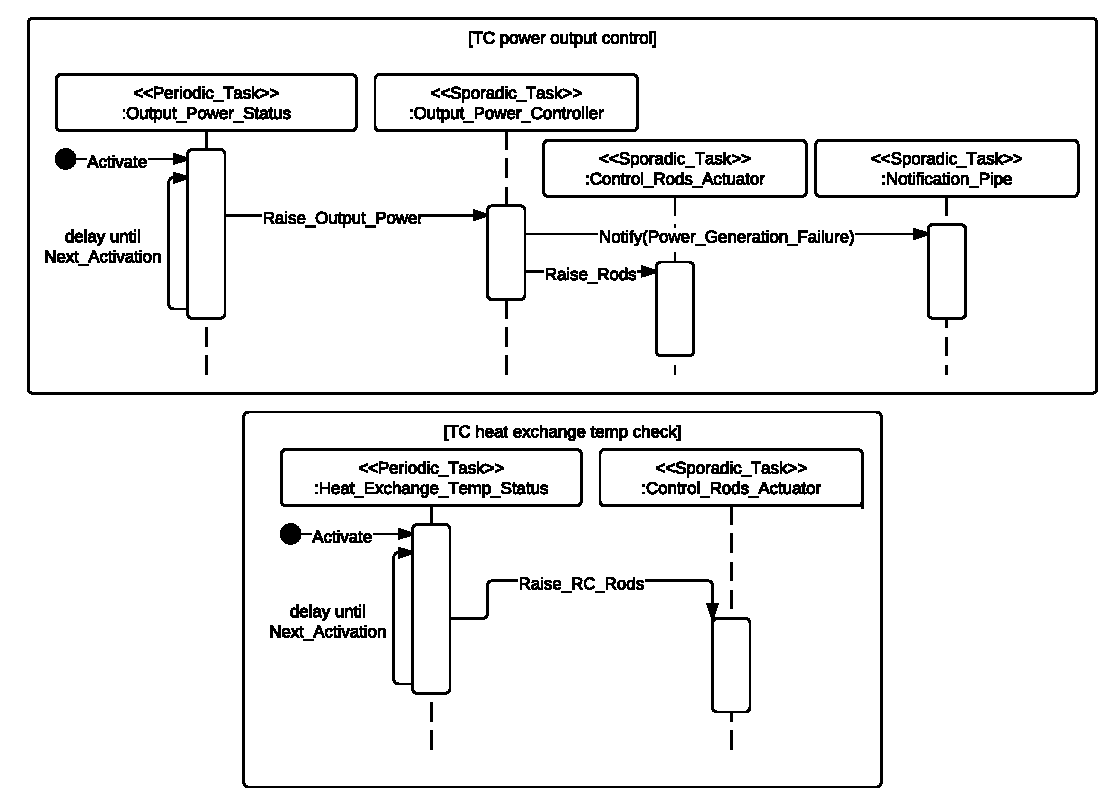
\includegraphics[width=\textwidth]{diagrams/TC_Status_Diagram1}
\caption{Heat exchange and output power checking tasks.}
\end{figure}
no direct communication between \texttt{Output\_Power\_Status} and control 
rods actuator task because we want to logically divide their duties, the first 
one just checks the correct functionality and the second checks if the plant 
support an output power raise and properly change shared data according to 
newly gathered informations. After that we have heat exchange temperature checks. 
If temperature is not high enough to convert water into steam communicate with 
control rods actuator task and request to raise them. Control rods are never 
raised above safety level. 

Some other controls are done in order to ensure punctual notifications of 
malfunctions. Two subsystems are checked periodically: TC\_Pump and cooling 
system. Once errors are detected start mode is switched to maintenance 
and users are notified. User notifications are important since there is no way 
to stem through software some kind of failures, such as these.
\begin{figure}[htb]
\centering
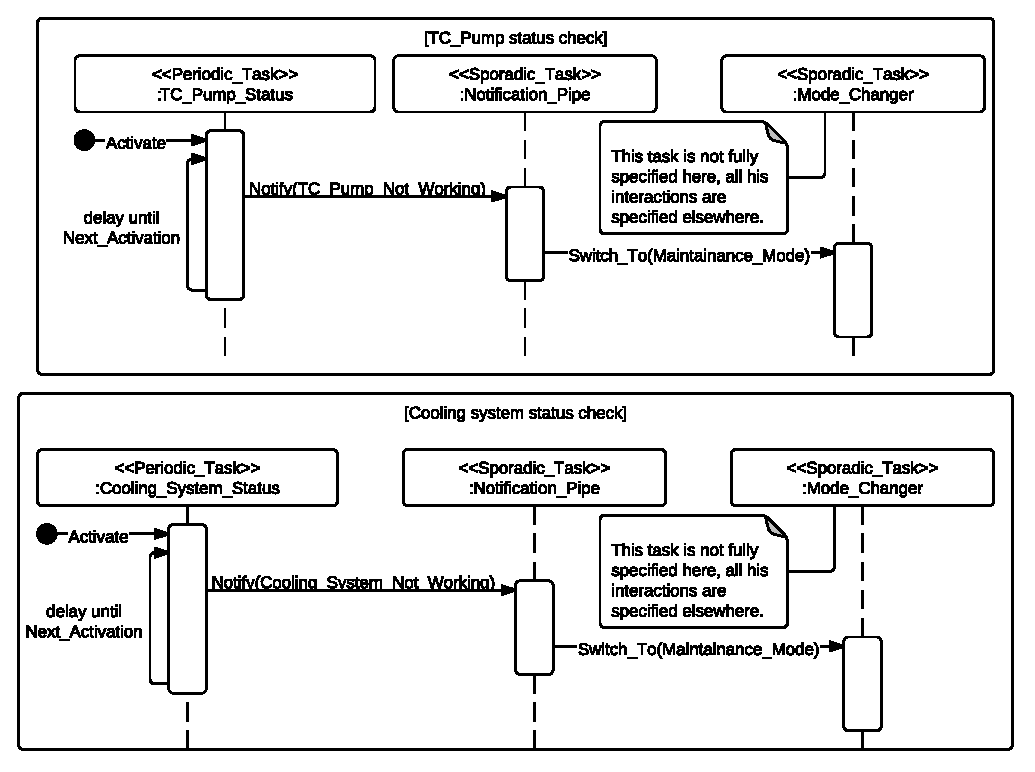
\includegraphics[width=0.8\textwidth]{diagrams/TC_Status_Diagram2}
\caption{TC pump and cooling system status-checking tasks}
\end{figure}
th 
% ------------------------------------------------------------------------------
% -- Periodic tasks recap table
% -- 
As done in previous section we present a recap table that enumerates periodic
non-critical tasks. For each task a simple description of its duty is given. This
helps understanding better the whole picture. 
\begin{table}[h!tb]
\centering 
\begin{tabular}{|l p{7cm}|}
\hline 
\textbf{Task} & \textbf{Duties} \\
\hline \hline
\texttt{Output\_Power\_Status} & Checks output power level and requests 
    \texttt{Output\_Power\_Controller} to raise it if it is too low for current 
    threshold.\\
\texttt{Heat\_Exchange\_Temp\_Status} & Checks that water temperature at heat 
    exchange with RC is high enough to ensure its transform into steam to allow
    plant operations. Request to raise control rods if it is not.\\
\texttt{TC\_Pump\_Status} & Checks functionality of TC\_Pump. If the pump do not
    responds as expected it notify to user and puts the plant into maintenance 
    mode.\\
\texttt{Cooling\_System\_Status} & Checks temperature of water after cooling. If
    it is too high notify to user a cooling system malfunction and put the 
    system into maintenance mode.\\
\hline
\end{tabular}
\caption{Periodic non-critical tasks recap table.}
\end{table}

% ------------------------------------------------------------------------------
% -- Sporadic tasks subsection
% --
\subsection{Sporadic tasks}
Here we will give an overview of remaining tasks. We will go more in details of
some tasks that has been met before and we will specify how they behave when 
stimulated. Some sporadic tasks has not to be further exploited since their 
behavior is dummy, i.e. actuator tasks just do what they are requested to do 
and performs simple feasibility checking of the actual operation.

One interesting and non-trivial task is \texttt{Notification\_Pipe} that exchange
message throughout the system and from/to users. This task awakes once exceptional
events happens, e.g. users require the plant to start its operations, and 
delivers messages to the right place. Another non-trivial task is 
\texttt{Mode\_Changer} that allow plant to go through its operational modes. 
Once it receive the signal to pass from a mode to another it notifies all of 
the tasks whether to activate or suspend with an appropriate 
protocol that aborts some tasks and lets some others finish. We discuss this
protocol in the next chapter.
\begin{figure}[htb]
\centering
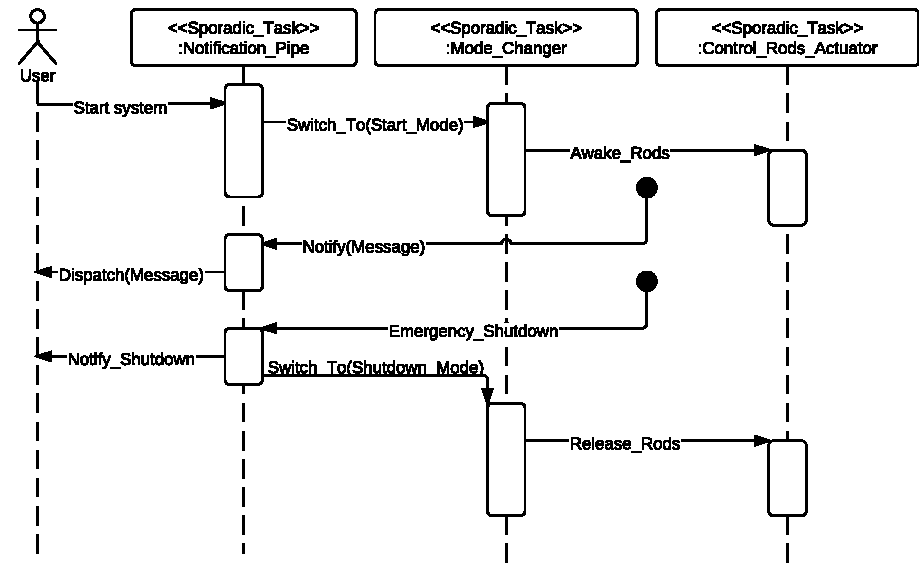
\includegraphics[width=0.9\textwidth]{diagrams/Mode_Changer}
\caption{
    Notification pipe sequence. Also some behavior of 
    \texttt{Mode\_Changer} are depicted here.
}
\end{figure}
We want to spend a few more words for \texttt{Output\_Power\_Controller} 
task. It allow plant to increase or decrease its power level production and manage 
turbines and generators. It knows what are the operational limits of the plant
and manages power production setting threshold values for other checking tasks. 
As usual we present a recap table to clarify which sporadic tasks we have and 
how they should behave.
\begin{table}[b]
\centering 
\begin{tabular}{|l p{7cm}|}
\hline 
\textbf{Task} & \textbf{Duties} \\
\hline \hline
\texttt{Control\_Rods\_Actuator} & Actuate control rods adjustments.\\
\texttt{RC\_Pressure\_Actuator} & Actuate RC water pressure adjustments.\\
\texttt{Notification\_Pipe} & Deliver notifications through the system.\\
\texttt{Mode\_Changer} & Change operational mode.\\
\texttt{Output\_Power\_Controller} & Raise or lower output power according to 
    requests.\\
\hline
\end{tabular}
\caption{Sporadic tasks recap table.}
\end{table}

% ------------------------------------------------------------------------------
% -- Task dependencies section
% --
\section{Task dependencies}
In this section we consider the relations between tasks. 
Figure \ref{depgraph} depicts those relations in a simple graph. We have not
considered shared resources yet, we present a wider overview diagram further on
in this document. Still, such diagram enable us to understand connections between
tasks. Those connections are inferred from previous specifications. A good 
architecture does not present cyclic dependencies: we designed the system with 
this constraint in mind.

One thing to notice while looking at task dependencies is that periodic tasks 
depend only on the clock. This is partially true since task \texttt{Mode\_Changer} 
that awakes periodic tasks is a dependency for those but we do not consider it. 
In general, we tolerate this because practically only the first job depend on 
\texttt{Mode\_Changer} while all the other do not. When we will perform analysis 
of the system we must take into account this assumption. This means that we 
analyze mode transitions and in-mode schedulability.
\begin{figure}[htb]
\centering
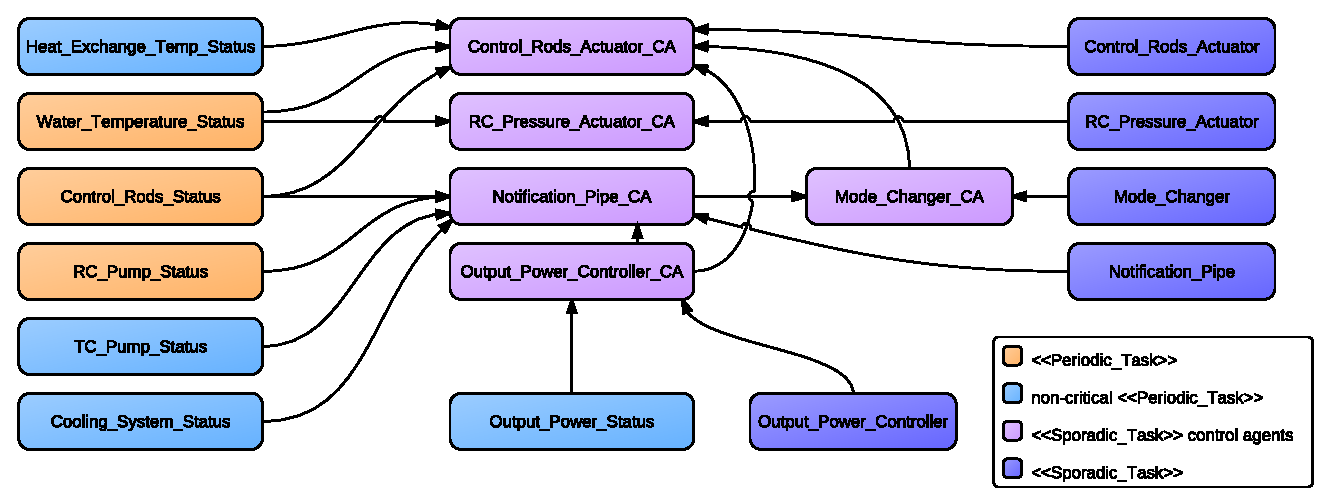
\includegraphics[width=\textwidth]{diagrams/Dependacy_Graph}
\caption{
    Task dependency graph. Connections represent resource usage, in the graph 
    are represented only control agents of sporadic tasks. All tasks also 
    use mode changer resources that are not represented here for readability.
}
\label{depgraph}
\end{figure}

% ------------------------------------------------------------------------------
% -- Resource management section
% -- 
\section{Resource management}
Up here we talked about system functionality without taking account shared 
resources. In this section we try to give an idea on how resources are managed. 

As shared resources, we have all of the actuators which has a related sporadic 
tasks that can be triggered upon requests. The actuator itself can be queried on its status. 
As an example we may call a procedure on control rods actuator resource that 
return current control rods status. Most resources in the system are managed 
this way. Physical actuators are all related to software actuators that can be 
queried for informations about the physical one. Some other resources that are not 
manageable by software (such as pumps) will have a dedicated protected resource 
that hides access to physical sensors. Once requested the resource will activate 
a data fetching procedure on the actual sensor. 

We introduce a notification daemon that periodically  send to user 
informations about the system. We need a server that listen and send informations
on the net to notify the user about current status. We use it also to 
receive user commands. So we have extended the system with other two tasks, we 
describe widely in next section how communication with users is carried out.

\begin{table}[htb]
\centering
\begin{tabular}{|l p{7cm}|}
\hline 
\textbf{Task} & \textbf{Duties} \\
\hline \hline
\texttt{Notification\_Daemon} & Periodically query plant apparatus and send 
    informations to user through \texttt{Net\_Server}. \\
\texttt{Net\_Server} & Send and receive messages from the net. Communicate with
    \texttt{Notification\_Daemon} and \texttt{Notification\_Pipe}.\\
\hline
\end{tabular}
\caption{User interaction tasks}
\end{table}

% ------------------------------------------------------------------------------
% -- User interaction section
% --
\section{User interaction}
As the purpose of this system is to be \emph{embedded}, users do not 
directly interact with it but will communicate commands to the system 
through the net with a simple protocol. User operations will be received and
managed by \texttt{Notification\_Pipe} that deliver the message to the 
intended recipient. The sending/receiving service is outside of core functionality 
and may be embodied, in the analysis, inside the notification subsystem as it talks 
and serves only the above-mentioned task. In the analysis we can assume that 
user input arrives at random time. We do not make any assumption on the net
communications, we just send notification to users in a UDP fashion. This
means that we send notifications without waiting for an ack. In the analysis we 
consider the task associated with the receiving of a packet as sporadic. It is 
activated by the arrival of a packet. 

\subsection{A simple protocol for user interaction}
Here we describe the protocol that we use in the system to exchange 
information between users and the system itself. Each message has an header that 
describes which type of message it is and what commands the message bears. We 
have just three type of messages: \texttt{USER\_CMD} refers that the 
message is to modify plant behavior; \texttt{NOTIFICATION} is a simple 
notification of system functionality; \texttt{CRITICAL\_NOTIFICATION} is 
when something has gone wrong and system notifies user that there are some 
things that users must do in order to restore operations. To deliver this
information we just need two bits, the rest of the header (6 bits) is used 
to specify further informations and commands. Table \ref{pktcmd} specifies
which commands are available.  
\begin{figure}[h!tb]
\centering
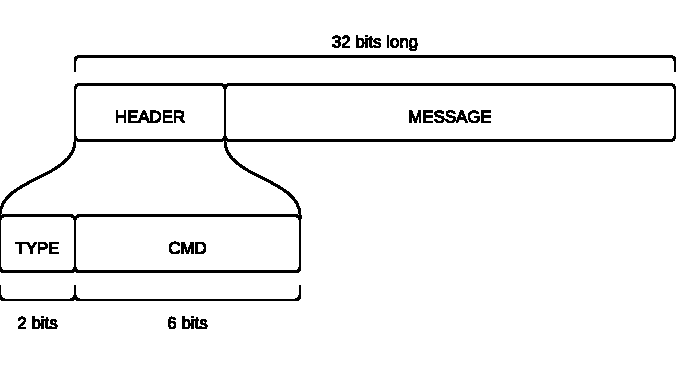
\includegraphics[width=0.65\textwidth]{images/Protocol}
\caption{Representation of a packet from user protocol}
\end{figure}
All the rest of the packet is a 24-bits selector that contains additional 
information about the error/command that has been notified.
We also give numeric codes for single instruction here because components may be 
written in different programming languages. Codes in the table are express in 
hexadecimal notation. Notifications has in the message part the informations that
they claim to carry. Further discussion about the protocol are found in appendix
\ref{app:protocol}

\section{Architecture summary}
Each component has been design to minimize coupling with others. The reader may
recall that each module of the architecture (except the physical one) 
contains tasks i.e. there are no empty modules and no task overlap between 
software layers. A small exception from a complete clear separation between 
layers is that periodic-status-checking tasks for turbine circuit are triggered 
by \texttt{Mode\_Changer}. Mode selection layer has been drawn above all other 
because has tight connection with both periodic non-critical tasks and 
notification subsystem. In the next chapter we discuss how this is actually 
carried out. We tolerate this exception since mode-change protocol is addressed 
separately in response-time analysis.
\begin{figure}[h!tb]
\centering
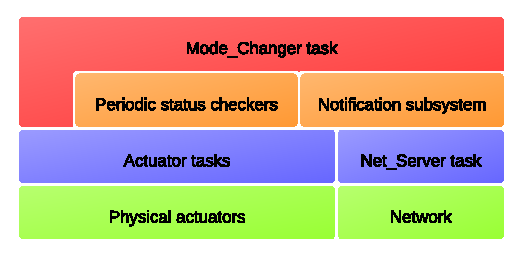
\includegraphics[width=0.65\textwidth]{images/ArchitectureOverview}
\caption{Architecture overview}
\label{fig:archover}
\end{figure}

% ------------------------------------------------------------------------------
% -- MODE-CHANGE PROTOCOL CHAPTER
% --
\chapter{Mode-Change Protocol}
In this chapter we present how mode changes are managed and the connections with 
response-time analysis. We first describe the protocol and how tasks behaves
during a mode-change transition. We also present an analysis on mode-change 
schedulability. We refer to \cite{real04} for the theoretical background that 
stands behind mode-change analysis and to \cite{real99} for the actual 
implementation. Hereafter we refer to a mode-change request with the acronym 
MCR as in \cite{real04}. Once a MCR is issued we do not accept other MCRs upon
the completion of mode-change transition. This means that the system double-checks
\texttt{Mode\_Changer} task, since it is a sporadic task it has a minimum
inter-arrival time and there is a minimum time between mode changes. 

\section{The Protocol}
First we need to present some notation that we use throughout the presentation
of the protocol. We call an \emph{old-mode completed} task one that is alive in 
the old-mode (before an MCR is issued) and is allowed to execute up to its 
completion in the transition. We call an \emph{aborted} task one that is 
immediately aborted upon an MCR. We call a \emph{new-mode changed} task one that 
is alive in the old mode and in the new mode, i.e. after the MCR, but changes its 
operation parameters. \emph{Wholly new} tasks are those that are introduced 
after the MCR and \emph{unchanged} tasks are also accepted. 

The protocol we use to manage mode changes is the one presented by Real in  
\cite{real04}. Assuming the MCR arrives at $t_{MCR}$ we have that:
\begin{itemize}
    \item Old-mode completed tasks are allowed to complete normally.
    \item Aborted tasks are immediately aborted at $t_{MCR}$.
    \item New-mode changed tasks have their first activation in the new mode 
          after a given offset $Y_i$. 
    \item Wholly new tasks are also introduced after an offset. 
    \item Unchanged tasks are preferably introduced without an offset. 
\end{itemize}
From this taxonomy follows table \ref{tbl:modechange} that presents how tasks 
in our system behave during a mode-change transition. Since we have almost the 
same behavior both in shutdown mode and maintenance mode we embody the four 
transitions into two in this presentation. What really changes  are the 
operational parameters. 

% ------------------------------------------------------------------------------
% -- TASKS BEHAVIOR ON MODE CHAGE - TABLE
% --
\begin{table}[htb]
\centering
\begin{tabular}{|r | p{35mm} | p{35mm}|}
\hline
& \textbf{SdM/MM to StM} & \textbf{StM to SdM/MM} \\

\hline 
\texttt{\small Control\_Rods\_Status}      & Unchanged & Unchanged \\
\texttt{\small Water\_Temperature\_Status} & Unchanged & Unchanged \\
\texttt{\small RC\_Pump\_Status}           & Unchanged & Unchanged \\

\texttt{\small Output\_Power\_Status}        & Wholly new & Aborted \\
\texttt{\small Heat\_Exchange\_Temp\_Status} & Wholly new & Aborted \\
\texttt{\small TC\_Pump\_Status}             & Wholly new & Aborted \\
\texttt{\small Cooling\_System\_Status}      & Wholly new & Aborted \\

\texttt{\small Control\_Rods\_Actuator}   & Unchanged & Unchanged  \\
\texttt{\small RC\_Pressure\_Actuator}    & Unchanged & Unchanged  \\
\texttt{\small Output\_Power\_Controller} & Wholly new & Aborted   \\
\texttt{\small Notification\_Pipe}        & Unchanged & Unchanged \\
\texttt{\small Mode\_Changer}             & Unchanged & Unchanged \\

\hline
\end{tabular}
\caption{
    Tasks behavior on mode change. SdM refers to shutdown mode, StM refers
    to start mode and MM refers to maintenance mode.
}
\label{tbl:modechange}
\end{table}

The actual implementation of the single task depends on its behavior during 
mode-change transition. This fact contrast with the archetypes given in the
previous chapter but can coexists with them. In \cite{real99}, Real and Wellings 
give a wide dissertation on the topic presenting some design pattern to follow 
in order to correctly implement mode change. Tasks that are unchanged are 
implemented using selective-accept statements. Abortable tasks are implemented 
using asynchronous transfer of control (ATC). Those facilities are found in Ada 
as part of the language semantics and in Real-time Java as part of its library. 

Here we present two code snippets from Real work \cite{real99}. The first refer
to non-abortable periodic tasks that can be easily adapted to sporadic tasks
adding a wait on a guarded entry. 
\begin{lstlisting}[frame=tb]
loop -- Non abortable periodic task
    select
        -- Mode change management is in this section
        Wait_Mode_Change(My_Current_Mode);
        Query_Mode_Change(My_Identity)
            (My_Current_Mode, Period, Next_Activation)
    or 
        -- Normal body of a periodic task
        delay until Next_Activation;
        Task_Start(My_Identity);
        if Current_Mode = My_Current_Mode then
            Job_Actions;
            Next_Activation := Next_Activation + Period;
        end if;
        Task_Stop(My_Identity);
    end select;
end loop;
\end{lstlisting}
The second snippet refers to abortable tasks and use ATC to manage abort. This 
code snippet can be transformed into a sporadic task performing the same 
operations described above. 
\begin{lstlisting}[frame=tb]
loop -- Abortable periodic task
    select
        Wait_Mode_Change(My_Current_Mode);
        Task_Stop(My_Identity, My_Current_Mode);
        Query_Mode(My_Identity)
            (My_Current_Mode, Period, Next_Activation);
    then abort
        loop -- Normal declaration of a periodic task
            delay until Next_Activation;
            Task_Start(My_Identity);
            Job_Actions;
            Next_Activation := Next_Activation + Period;
            Task_Stop(My_Identity, My_Current_Mode);
        end loop;
    end select;
end loop;
\end{lstlisting}
The reader may notice that the two patterns have a slight difference so that 
the first has just one loop that embodies the whole selective-accept statement 
and the second has also an inner loop. Their behavior is as expected: in the 
first scenario every period will execute normally and operational parameters 
will be modified on mode change. In the second scenario tasks loop while the 
guarded entry is closed; once the guard is opened the inner loop is aborted.

For completeness in Real-time Java ATC can be managed through 
\texttt{AsyncEvent} and \texttt{AsyncEventHandler} 
classes that may invoke \texttt{interrupt()} on the abortable task that must be 
of type \texttt{RealtimeThread} (from \cite{brosgol02}). 

\section{Protocol Analysis}
The whole analysis is carried out with the assumption that the software system
runs on a single processor using fixed priority scheduling policy and ceiling 
locking (ICPP, immediate ceiling priority protocol) for resource access. 
What we want to point out here is which task interfere with each other 
and how to control this interference.

We divide the analysis in old-mode tasks response time and new-mode tasks response 
time. The first (old-mode tasks) suffers more interference from new-mode changed
and wholly new tasks with higher priorities. Since we want to allow only 
critical tasks to be alive through all operation modes these have the highest 
priority in order to suffer less interference possible. New-mode changed and 
wholly new tasks suffers more interference from unchanged tasks. Real presents
also an algorithm to calculate offsets in order to maximize schedulability of 
the mode-change transitions. At the end of the response-time analysis of the 
single modes we should give an estimation of the offsets to use. 

% ------------------------------------------------------------------------------
% -- System Analysis chapter
% -- 
\chapter{System Analysis}
In this chapter we report the analysis done for the system. First we explain how
the analysis has been carried out, which instruments have been used in order to
ensure reliable results. Second we introduce what are analysis 
parameters and how they are changed in different scenarios. Finally we present 
the result of the above-mentioned analysis. The whole analysis is carried out
with the hypothesis of a single-core fixed priority processor and immediate 
ceiling priority protocol to manage shared resources. We analyze the various 
operation modes separately. 

\section{Instruments and Techniques}
We used MAST (Modeling and Analysis Suite for Real-Time Applications) to perform 
the analysis task. MAST is a big tool and we used a little part of it, for 
further informations see \cite{gonzalez01}. 
Our analysis process is: 
\begin{itemize}
    \item A configuration file which specifies CPU and tasks parameters is used
    from MAST. All of the files created share a common template, the reader may
    find this template in appendix \ref{app:masttemplate}.
    \item MAST is run with appropriate file as input. Results are stored in an 
    output file. All modes are analyzed separately.
    \item The process is repeated over different scenarios changing operation 
    parameters in order to track changes in response times and schedulability. 
\end{itemize}
Priority assignment and WCETs are calculated by MAST. Since the aim of this 
project is to perform a research on the topic our WCETs are not realistic but 
give us an estimation. Given a CPU with $f$ clock frequency and $r_{cpi}$ 
worst-case cycles per instruction ratio, a task with $s$ source lines of code 
(SLOC) and a compiler that has $r_{asm}$ worst-case machine operations over 
source lines of code ratio we calculate WCET as follow:
\[
    t_{WCET} = \frac{(s \cdot r_{asm}) r_{cpi}}{f}
\]
We use \texttt{Speed\_Factor} of the \texttt{Processing\_Resource} object to 
calculate WCET. Given the previous equation, we set in the MAST specification 
WCETs for tasks as if they were SLOC and the speed factor to:
\[
    sf = \frac{f}{r_{asm} * r_{cpi}}
\]
This allow us to change just the speed factor parameter in order to switch 
from a CPU type to another one. It is the inverse of the previous equation since
WCETs are divided by speed factor in MAST. 

We also let MAST calculate priorities as well as resource ceilings.
Priorities are generated using deadline monotonic assignment within the range 
$[1, 10]$.
Analysis is done using offset-based technique that support also distributed 
systems but produce good results also for mono-processor ones.
 
\subsection{Task description}
While analyzing the system with MAST we need to formalize it with a specific 
description of all of its tasks (that are mapped to transactions), 
jobs (that are mapped to operations), shared resources and processors. In this 
section we give a precise idea on how the system has been described formally to
be analyzed. Figure \ref{fig:mstartjob} depict system jobs in 
\begin{figure}[htb]
\centering 
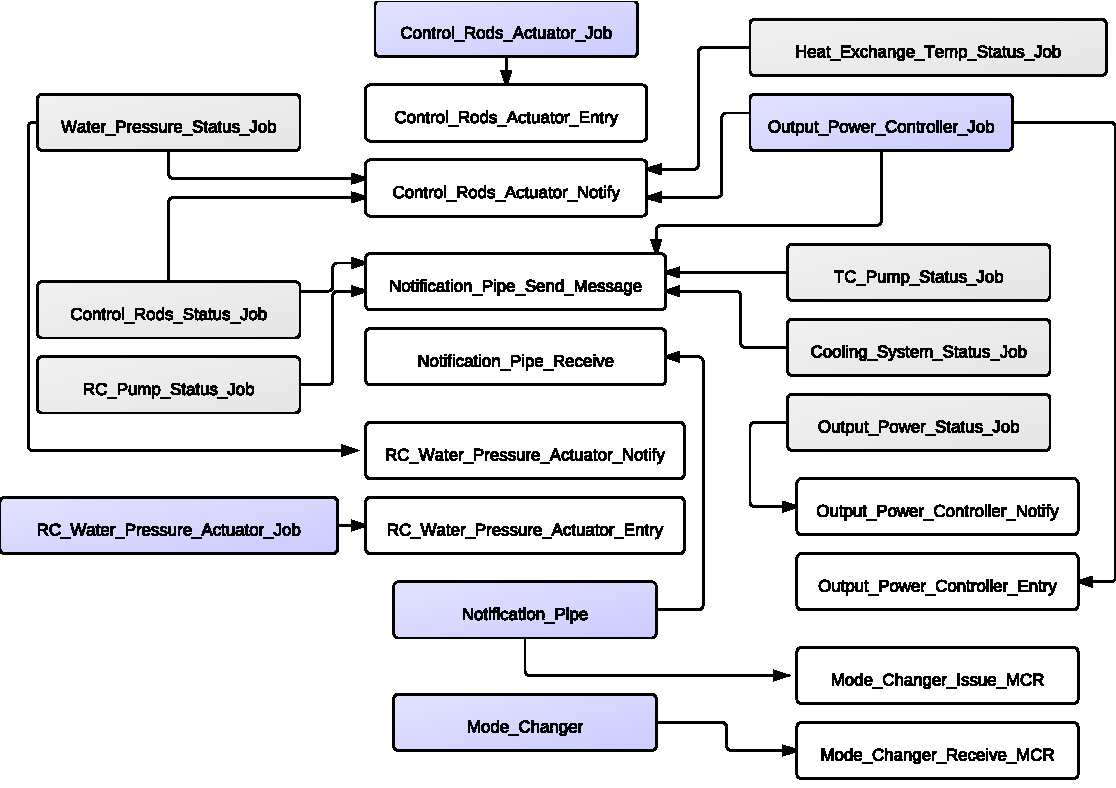
\includegraphics[width=\textwidth]{diagrams/Transactions}
\caption{
    System operations (i.e. jobs) and their connections for \emph{start mode}.
    Light gray colored operations are issued by periodic tasks and light blue 
    ones are issued by sporadic tasks. 
}
\label{fig:mstartjob}
\end{figure}
\emph{start mode} as it is represented into the MAST description we created. 
Each of the rectangle in figure is an operation, the white ones are simple and
they use a shared resource and the colored ones are enclosing operations. If an
arrow connects an enclosing operation to a simple one (this is the only 
direction allowed, there is no arrow from simple to enclosing) it means that 
that enclosing operation use the simple operation. The reasoning behind this 
subdivision is that simple operations maps critical sections (i.e. entry or 
procedures in protected resources) and the enclosing operations are jobs that
are issued by task. Indeed tasks are mapped to MAST transactions. Figure 
\ref{fig:masttrans} depicts this mapping. Each tasks is a regular transaction in 
MAST the difference stands in which type of event is its trigger. For periodic 
tasks the events that initiate the transactions are periodic and for sporadic 
tasks events are sporadic. At the end, all of the tasks have hard timing 
constraints i.e. we specified for all of the transactions an 
\texttt{Hard\_Global\_Deadline}. The same goes for \emph{maintenance and 
shutdown modes} that are depicted in figure \ref{fig:mmmode}, in appendix 
\ref{app:masttemplate} it is listed the template file we used to generate all 
of the scenarios. The template is for start mode, the main difference between it 
and the maintenance and shutdown one is that some of the operations and 
transitions are not present. 
\begin{figure}[htb]
\centering 
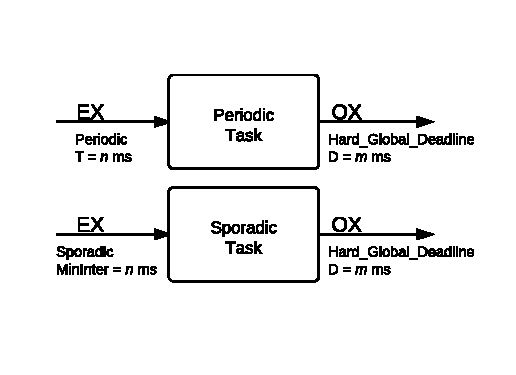
\includegraphics[width=0.65\textwidth]{diagrams/TransMAST}
\caption{Task/transaction mapping in MAST.}
\label{fig:masttrans}
\end{figure}

\begin{figure}[htb]
\centering 
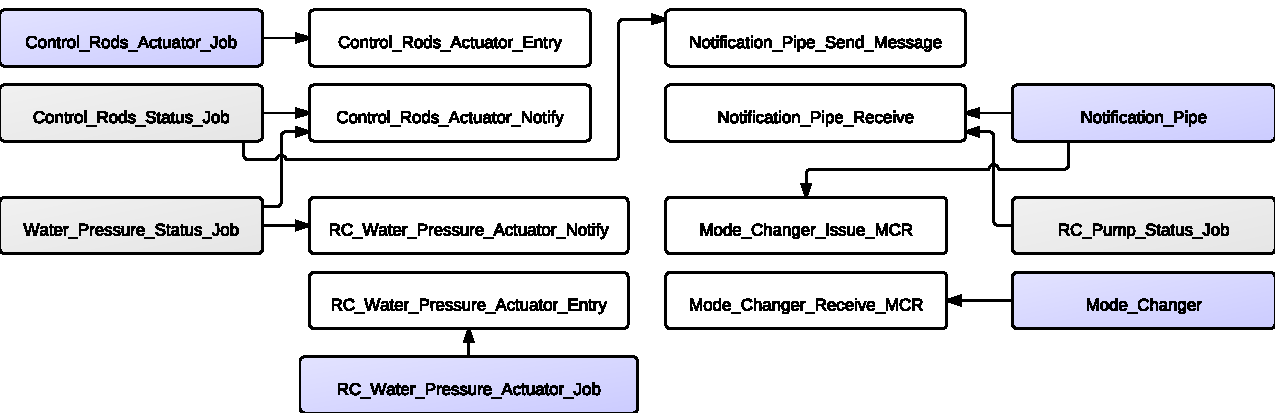
\includegraphics[width=\textwidth]{diagrams/TraMM}
\caption{System operations for \emph{maintenance and shutdown} modes.}
\label{fig:mmmode}
\end{figure}

\section{Analysis scenarios}
In this section we list all of the parameters for each analysis scenario. First
we will introduce what are tasks parameters, then we enumerate which processors 
we use to perform the analysis.

\subsection{Task Parameters}
Here we overview what are the invariant tasks parameters that we use
in the analysis. For each task we identify some parameters as constituent. 
Those parameters do not change across the different analysis scenarios. They are:
source lines of code that express the dimension of the task to perform; if the 
task is periodic or sporadic; which shared resources the task will use. The 
shared resources used are important since they will have a ceiling associated 
with it and this ceiling will be calculated from the priorities of the task that
are using that particular resource. 
\begin{table}[tb]
\makebox[\textwidth][c]{
\begin{tabular}{|r | c c l|}
\hline
\textbf{Task} & \textbf{SLOC} & \textbf{Periodic} & \textbf{Shared Resources}\\
\hline

\texttt{Control\_Rods\_Status}   & 200 & Yes & CRA\_CA, NP\_CA \\
\texttt{RC\_Pump\_Status}        & 200 & Yes & NP\_CA \\
\texttt{Water\_Pressure\_Status} & 200 & Yes & CRA\_CA, RCPA\_CA \\

\texttt{Heat\_Exchange\_Temp\_Status} & 120 & Yes & CRA\_CA \\
\texttt{Output\_Power\_Status}        & 120 & Yes & OPC\_CA \\
\texttt{TC\_Pump\_Status}             & 120 & Yes & NP\_CA \\
\texttt{Cooling\_System\_Status}      & 120 & Yes & NP\_CA \\

\texttt{Control\_Rods\_Actuator}   & 150 & No & CRA\_CA \\
\texttt{RC\_Pressure\_Actuator}    & 150 & No & RCPA\_CA \\
\texttt{Output\_Power\_Controller} & 150 & No & OPC\_CA, CRA\_CA, NP\_CA \\
\texttt{Notification\_Pipe}        & 500 & No & NP\_CA, MC\_CA \\
\texttt{Mode\_Changer}             & 350 & No & MC\_CA \\
\hline
\end{tabular}
}
\caption{
    Constituent parameters of task set. SLOC stands for source lines of code.
    This parameters are fixed for each operation mode. For a full list of 
    correspondence between the acronym and the shared resource that it represent
    see table \ref{resacronym}. 
}
\end{table}

Parameters that are typical of a test scenario are deadline and period. For 
sporadic task we will refer to their minimum inter-arrival not to their period. 
Varying those parameters we can obtain a feasible (or not) scheduling for our 
system. We present here another table with the various analysis scenarios. We 
designed those scenarios trying to push system to 100\% of utilization. 
Shutdown mode and maintenance mode have been analyzed together due to they use 
the same tasks. 

Looking at table \ref{tbl:scenariodef} the reader may notice that each scenario 
is more restrictive (in terms of timing constraints) than the previous one. When 
we discuss analysis results we use this information in order to make some 
observations on the system. 

\emph{Maintenance and shutdown mode} have been analyzed together. First we used 
the same scenarios used for start mode to see what changes removing some tasks 
then we tailored a scenario that try to maximize schedulability in this mode. We
present this scenario in the table \ref{tbl:scenariomm}.

\subsection{Processors specification}
We evaluate the system over four different processors. Two that has a frequency 
of 20MHz and 5 cycles per instruction but the first requires 4000 machine 
operations for context switch and the second only 2000 machine 
operations to do the same. Then we evaluate two CPUs that has 100Mhz as clock 
speed at 2 cycles per instructions and, respectively, 4000 and 2000 machine 
operations for context switch. Times have been normalized to processor 
speed with \texttt{Speed\_Factor} since MAST accept time for worst-case context 
switch in normalized unit. Normalized time is obtained multiplying speed factor 
by actual time.
We perform the analysis on different processor in order to estimate what are 
the most influential parameters that heavily change results in schedulability. 
\begin{table}[h!tb]
\centering
\begin{tabular}{|r lll|}
    \hline
    \textbf{\#} & \textbf{Frequency} & \textbf{CPI} & \textbf{WCS} \\
    \hline
    1 & 20MHz  & 5 & 1ms    \\
    2 & 20MHz  & 5 & 0.5ms  \\
    3 & 100Mhz & 2 & 0.08ms \\
    4 & 100Mhz & 2 & 0.04ms \\
    \hline
\end{tabular}
\caption{
    Processors recap table. Please note that the worst-case context switch is
    given in milliseconds and its calculated with the actual parameters of the
    current processor.  
}
\end{table}

\section{Analysis Results}
In this section we preset the results of the analysis. First we want to do some
consideration on the overall schedulability of the given task set and then we 
go deeper into considering the \emph{sustainability} and the \emph{sensitivity} 
results. 

For \emph{start mode} the system is schedulable in all of the scenarios designed. 
The data collected shows that, for our system, the WCS greatly influence system 
schedulability. Worst-case context switch is one of the parameters to take into 
account while designing a real-time software system. We also tested different 
policy for resource allocation (using the POSIX option of MAST) but the results 
were the same as using strict ICPP.

For \emph{maintenance and shutdown mode} considerations are tightly similar 
since they are relaxations of the system i.e. there are less active tasks, 
the system is sustainable and remain schedulable. 
We discuss more about system sustainability in the next section. 

\subsection{Sustainability}
One interesting consideration on the analysis is about system sustainability. The
system is sustainable if any relaxation preserve schedulability. Our analysis 
show that the relaxation effectively preserve schedulability and, due to the 
nature of fixed-priority scheduling together with ICPP, the overall behavior of 
a single scenario is the same on every CPU. We present a couple of plots that 
prove our statements. Figure \ref{fig:periodic} shows the average behavior of 
periodic tasks on different CPUs. From this plot we see that average response 
time is shifted depending on the speed (that take account both of CPU frequency
and WCS). We notice the same facts for sporadic tasks. The slope in the plot 
are decreasing because the WCET is the same in every scenario and what changes 
are the deadlines. This result in a higher response time since tasks are 
scheduled with a lower priority with deadline monotonic priority assignment.

\begin{figure}[tb]
\centering
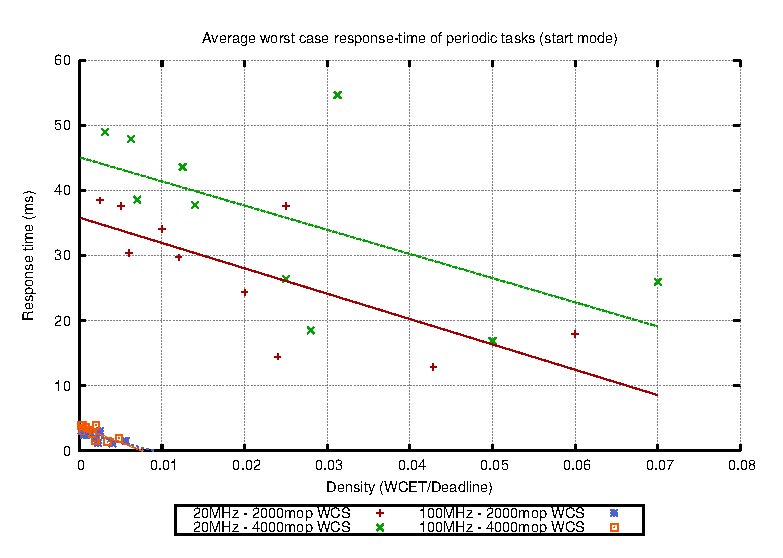
\includegraphics[width=\textwidth]{plots/sust_periodic}
\caption{
    Comparison of periodic tasks running over different CPUs in \emph{start 
    mode}. The reader may notice that slopes are shifted due to faster 
    processors and shorter WCS. \emph{mop} stands for machine operations. 
}
\label{fig:periodic}
\end{figure}

Figure \ref{fig:sporact} and 
\ref{fig:sporserv} shows the comparison of sporadic tasks over different CPUs.
We split the plot into two separate for readability. 
In those plots we compared on the density (that is calculated as $d=\frac{C_i}{D_i}$) 
rather than minimum interarrival time or other data because both worst-case 
execution time and deadline fully determine task behavior in the system (if the 
minimum interarrival time is less than the deadline, which is often the case). The 
same reasoning done over periodic task may be done here. The plots are less 
obvious to read than the previous one but the fact that is notable is that 
the shape that is found for each task is shifted when they run on different 
processors. The distance between the same point on the shape on different 
scenarios tell us what is the performance gain of choosing one or another CPU. 
One interesting fact to notice is that relaxing deadlines and minimum 
interarrival time result in an improved reactivity for sporadic tasks. The 
reader may see that the more the system is relaxed the more sporadic task has a 
lower response-time. 

These results were expected since it has been shown (see \cite{burns08}) that 
the approach we adopted (single fixed-priority processor and ICPP for resource 
sharing in a sporadic workload) is sustainable. 
\begin{figure}[p]
\centering
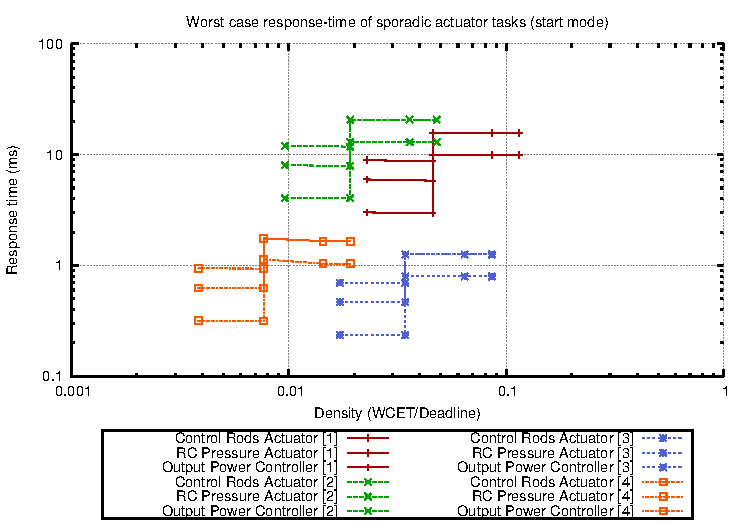
\includegraphics[width=0.87\textwidth]{plots/sust_sporadic_act}
\caption{
    Comparison of sporadic tasks that act as actuator running over different CPUs
    in \emph{start mode}. Please note that the scale of the axis is 
    logarithmic. In this plot (1) refer to 20Mhz/2000mop WCS, (2) to 20MHz/4000mop WCS, 
    (3) to 100Mhz/2000mop WCS and (4) to 100MHz/4000mop WCS.
    Each task set on different processor is scheduled the same way, the reader may
    notice that each shape is shifted in a different way over the plot. This is a
    prove of sustainability of FPS together with ICPP.
}
\label{fig:sporact}
\end{figure}

\begin{figure}[p]
\centering
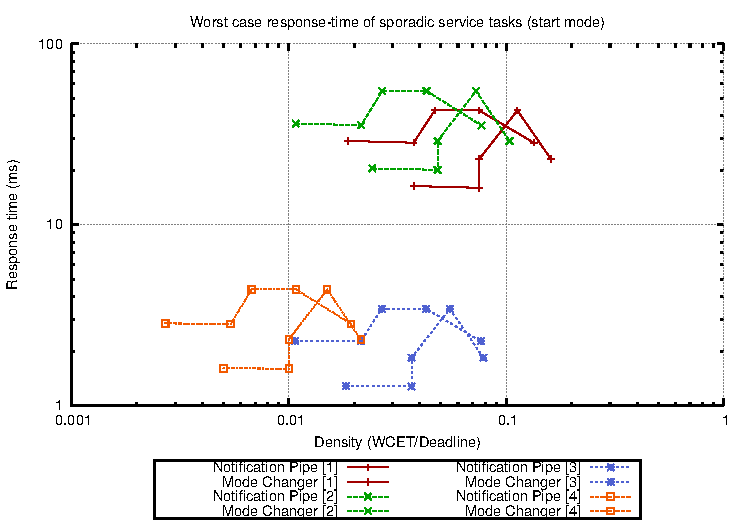
\includegraphics[width=0.87\textwidth]{plots/sust_sporadic_ser}
\caption{
    Comparison of sporadic tasks that provide system services running over 
    different CPUs in \emph{start mode}. Please note that the scale of the
    axis is logarithmic. In this plot (1) refer to 20Mhz/5ms WCS, (2) to 
    20MHz/1ms WCS, (3) to 100Mhz/5ms WCS and (4) to 100MHz/1ms WCS. The same 
    reasoning done in previous case may be extended here. Task on different 
    CPUs react differently but maintain the same overall behavior. 
}
\label{fig:sporserv}
\end{figure}

\subsection{Sensitivity}
Sensitivity analysis allow us to understand how changes of sensitive parameters 
of a single task affect overall system behavior. What we did here is to choose 
a scenario and change a single parameter over some range and see how the system
behaves. In figure \ref{fig:senseper} we depict how slack changes when deadline 
changes. We tested this property on three different tasks, first we chose a 
periodic task (\texttt{Control\_Rods\_Status}) and changed its deadline to see 
how the system reacts to this change and then we did the same for two sporadic task
(\texttt{Control\_Rods\_Actuator} and \texttt{Notification\_Pipe}). Obviously, 
while testing a single task all of the other parameters were not changed. We used
scenario 3 and the CPU with 20Mhz and 1ms of WCS as testbed. 

The plot in figure \ref{fig:senseper} may confuse the reader since the relation 
that stands behind response time analysis is not linear but its a fix-point. The 
different tests showed indeed that depending on the task the resulting slope (by 
task) is different but, the overall system slack grows almost linearly with the 
relaxation of the single parameter.

\begin{figure}[tb]
\centering
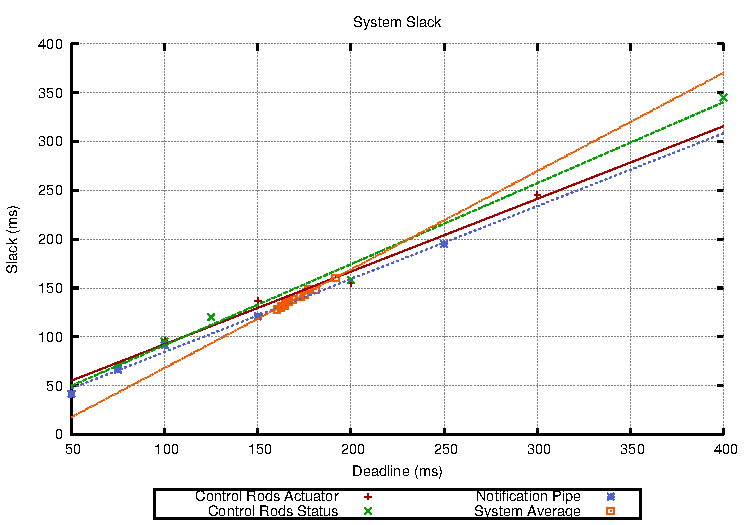
\includegraphics[width=0.95\textwidth]{plots/sense_slack}
\caption{
    Slack compared on deadlines. Each slope has been obtained varying the 
    deadline of that task letting the other parameters not to change. Each 
    slope is by itself a linear increase of slack for the task but globally 
    this is not true since the response-time analysis equations are 
    fix-point equations. 
}
\label{fig:senseper}
\end{figure}

Another aspect we decided to analyze is how variations in shared resource 
utilization affect schedulability. Figure \ref{fig:sensespo} shows how slack 
(and consequently response time) changes for tasks that use that particular 
resource (in this case is \texttt{Control\_Rods\_Actuator\_Control\_Agent}). 
Fixed all other parameters we changed the WCET of methods that act over shared 
resources (in MAST we specified longer critical sections). What we see is that 
the increasing usage of the resource affect response time of tasks that use that 
resource and may lead to an unfeasible scheduling soon. In essence what we want 
to point out is that the increasing WCET of the critical section exponentially 
affect system schedulability because all of the tasks that use that resource will
suffer longer blocking times and consequently have longer response times. 
If all of the $n$ tasks that share a resource share also a common critical 
instant what we obtain is that if WCET of critical section increase this 
increase will affect $n$ times on response time of the lower priority task.
This can be noticed also from previous plots. Plots \ref{fig:sporact} and 
\ref{fig:sporserv} has logarithmic scale, this is because the growth of the 
distance compared to the WCET is exponential. 

\begin{figure}[htb]
\centering
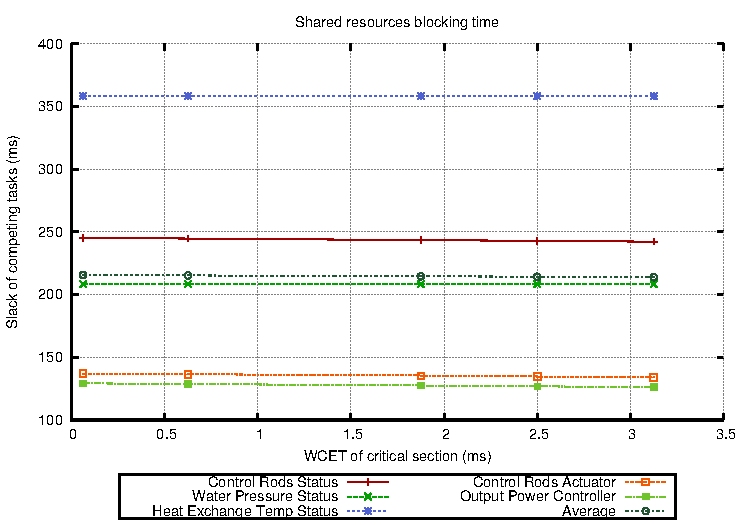
\includegraphics[width=\textwidth]{plots/sense_wcet}
\caption{
    Worst case execution time of critical section sensitivity. WCET of 
    \texttt{Control\_Rods\_Actuator\_Control\_Agent} critical section has been 
    changed over the range depicted to study changes in response time and slack.
    The overall slack does not suffer much from critical section growth on the 
    contrary response time suffers the most in percentage.
}
\label{fig:sensespo}
\end{figure}


% ------------------------------------------------------------------------------
% -- User protocol specification appendix
% -- 
\appendix
\chapter{User Protocol Specification} \label{app:protocol}

\begin{table}[htb]
\centering
\begin{tabular}{|l l|}
% -- User commands
\hline
\textbf{User commands} & \\ \hline \hline
\textbf{Code} & \textbf{Description}\\
\hline
\texttt{000} & Emergency shutdown \\
\texttt{001} & Switch to shutdown mode \\
\texttt{002} & Switch to operational mode \\
\texttt{003} & Switch to maintenance mode \\
\hline

% -- Notifications
\textbf{Notifications} & \\ \hline \hline
\textbf{Code} & \textbf{Description}\\
\hline
\texttt{000} & Control Rods status \\
\texttt{001} & RC water pressure \\
\texttt{002} & RC pump water temperature \\ 
\texttt{003} & RC pump pressure \\
\texttt{004} & Current output power \\
\texttt{005} & Water temperature at cooling\\
\texttt{006} & Heat exchanger temperature  \\
\texttt{007} & TC pump temperature \\
\texttt{008} & TC pump pressure \\
\texttt{009} & Turbine RPM \\
\texttt{00A} & Water pressure at turbine \\
\hline

% -- Critical notifications
\textbf{Critical Notifications} & \\ \hline \hline
\textbf{Code} & \textbf{Description}\\
\hline
\texttt{000} & Emergency Shutdown started \\
\texttt{001} & RC pump is not working \\
\texttt{002} & TC pump is not working \\ 
\texttt{003} & Cooling system failure \\
\texttt{004} & Pressure controller is not working \\
\texttt{005} & Turbine group failure \\
\hline

\end{tabular}
\caption{Available commands in user protocol}
\label{pktcmd}
\end{table}

\chapter{Tables}

\section{Analysis scenarios}
% ------------------------------------------------------------------------------
% -- Scenario definitions.
%\ --
\begin{table}[hbt]
\makebox[\textwidth][c]{

\begin{tabular}{|l | *{5}{|r|} *{5}{|r|}}
\hline
\textbf{Task} & \multicolumn{5}{c||}{\textbf{Deadline}} 
              & \multicolumn{5}{c|}{\textbf{Inter-arrival Time}} \\
\hline 
\multicolumn{1}{|r||}{\textbf{Scenario \#}} 
    & \textbf{1} & \textbf{2} & \textbf{3} & \textbf{4} & \textbf{5}
    & \textbf{1} & \textbf{2} & \textbf{3} & \textbf{4} & \textbf{5} \\
\hline
% -- Periodic critical tasks ---------------------------------------------------
\texttt{Control\_Rods\_Status}   & 500 & 250 & 125 & 70 & 50 
                                 & 500 & 250 & 125 & 70 & 50\\
\texttt{RC\_Pump\_Status}        & 500 & 250 & 125 & 70 & 50
                                 & 500 & 250 & 125 & 70 & 50\\
\texttt{Water\_Pressure\_Status} & 500 & 250 & 125 & 70 & 50
                                 & 500 & 250 & 125 & 70 & 50 \\                        
% -- Periodic non-critical tasks -----------------------------------------------

\texttt{Heat\_Exchange\_Temp\_Status} & 800 & 400 & 200 & 100 & 80
                                      & 800 & 400 & 200 & 100 & 80 \\
\texttt{Output\_Power\_Status}        & 800 & 400 & 200 & 100 & 80
                                      & 800 & 400 & 200 & 100 & 80 \\
\texttt{TC\_Pump\_Status}             & 800 & 400 & 200 & 100 & 80
                                      & 800 & 400 & 200 & 100 & 80 \\
\texttt{Cooling\_System\_Status}      & 800 & 400 & 200 & 100 & 80
                                      & 800 & 400 & 200 & 100 & 80 \\                   
% -- Sporadic tasks ------------------------------------------------------------

\texttt{Control\_Rods\_Actuator}   & 300  & 150  & 150 & 80  & 60
                                   & 2000 & 1000 & 500 & 300 & 250\\
\texttt{RC\_Pressure\_Actuator}    & 300  & 150  & 150 & 80  & 60
                                   & 2000 & 1000 & 500 & 300 & 250\\
\texttt{Output\_Power\_Controller} & 300  & 150  & 150 & 80  & 60
                                   & 2000 & 1000 & 500 & 300 & 250\\
\texttt{Notification\_Pipe}        & 300  & 150  & 150 & 100 & 70
                                   & 1000 & 500  & 250 & 250 & 150\\
\texttt{Mode\_Changer}             & 500  & 250  & 250 & 125 & 70 
                                   & 2000 & 1000 & 500 & 500 & 250\\
\hline
\end{tabular}
}
\caption{
    List of system analysis scenarios for \emph{start mode}. Inter-arrival time 
    refers to period for periodic tasks and to minimum inter-arrival time for 
    sporadic tasks. This table does not exploit all the dependencies between 
    tasks. For the whole specification refer to appendix \ref{app:masttemplate}.
}
\label{tbl:scenariodef}
\end{table}


\begin{table}[htb]
\begin{tabular}{|r |l l|}
\hline
\textbf{Task} & \textbf{Deadline} & \textbf{Inter-arrival Time} \\
\hline
\texttt{Control\_Rods\_Status}   & 340 & 340\\
\texttt{RC\_Pump\_Status}        & 340 & 340\\
\texttt{Water\_Pressure\_Status} & 340 & 340\\

\texttt{Control\_Rods\_Actuator}       & 150 & 800 \\
\texttt{RC\_Water\_Pressure\_Actuator} & 150 & 800 \\
\texttt{Notification\_Pipe}            & 200 & 700 \\
\texttt{Mode\_Changer}                 & 350 & 800 \\
\hline
\end{tabular}
\caption{\emph{Maintenance and shutdown} mode special scenario.}
\label{tbl:scenariomm}
\end{table}

\newpage

\section{Shared Resource Acronym}
\begin{table}[h!tb]
\centering
\begin{tabular}{|l | l|}
\hline
\textbf{Resource} & \textbf{Acronym} \\
\hline
\texttt{Control\_Rods\_Actuator\_Control\_Agent}   & CRA\_CA  \\
\texttt{RC\_Pressure\_Actuator\_Control\_Agent}    & RCPA\_CA \\
\texttt{Output\_Power\_Controller\_Control\_Agent} & OPC\_CA  \\
\texttt{Notification\_Pipe\_Control\_Agent}        & NP\_CA   \\
\texttt{Mode\_Changer\_Control\_Agent}             & MC\_CA   \\
\hline
\end{tabular}
\caption{
    This tables holds correspondence between shared resources and their acronyms.
    We use the acronyms for sake of brevity. 
}
\label{resacronym}
\end{table}


\section{Worst-Case Execution Times}
\begin{table}[h!tb]
\centering
\begin{tabular}{|r|l l|}
\hline

\textbf{Task} & \textbf{20MHz(5cpi)} & \textbf{100MHz(2cpi)} \\
\hline

\texttt{Control\_Rods\_Status}   & 2.5ms & 0.2ms \\
\texttt{RC\_Pump\_Status}        & 2.5ms & 0.2ms \\
\texttt{Water\_Pressure\_Status} & 2.5ms & 0.2ms \\

\texttt{Heat\_Exchange\_Temp\_Status} & 1.5ms & 0.12ms \\
\texttt{Output\_Power\_Status}        & 1.5ms & 0.12ms \\
\texttt{TC\_Pump\_Status}             & 1.5ms & 0.12ms \\
\texttt{Cooling\_System\_Status}      & 1.5ms & 0.12ms \\

\texttt{Control\_Rods\_Actuator}   & 1.875ms & 0.15ms \\
\texttt{RC\_Pressure\_Actuator}    & 1.875ms & 0.15ms \\
\texttt{Output\_Power\_Controller} & 1.875ms & 0.15ms \\
\texttt{Notification\_Pipe}        & 6.25ms  & 0.5ms  \\
\texttt{Mode\_Changer}             & 4.375ms & 0.35ms \\

\hline
\end{tabular}
\caption{
    WCET for each task calculated on different processors, here we do not
    include context switch. In the analysis it has been taken into account 
    also the context switch. 
}
\label{tbl:wcet}
\end{table}

\chapter{MAST template file} \label{app:masttemplate}
\lstinputlisting[language=mast, frame=tb]{sources/template.mast}


\bibliographystyle{plain}
\bibliography{bib}

\end{document}

